\documentclass[main.tex]{subfiles}

\begin{document}
The Gui is divided in two main sections:
\begin{itemize}[noitemsep]
\item The instrument grid
\item The side bar
\end{itemize}
The Instrument Grid is composed by an arbitrary number of slots, which can contain an instance of an instrument. The type of instrument can be selected through a drop down menu.\\
[2mm]
Each instrument, shows some specific parameters that act on the temporal and timbral characteristics of the sound, and a sequencer section that is common among all the instruments.\\
[2mm]
The sequencer section contains all the parameters useful for setting an euclidean sequence to the selected instrument, a humanizer knob, and a volume knob. 
As far as the Euclidean sequence is concerned, the step knobs, sets the length of the rhythmic sequence in terms of sixteenth notes; the hits knob sets the number of onsets, to distribute as evenly as possible in the sequence, according to the Euclidean algorithm. Finally, the offset knob allows the sequence to rotate, to achieve all the possible rotation of the same Euclidean rhythm.
The humanizer knob can be used to specify the amount by which every onset in the sequence is shifted apart with respect to their precise location, in order to simulate a human behaviour.
The volume knob simply allows to adjust the amplitude of each sound generated.\\
[2mm]
The Side Bar is used to set the global tempo in beat per minutes.\\
[2mm]
\begin{figure}[htbp]
\centering
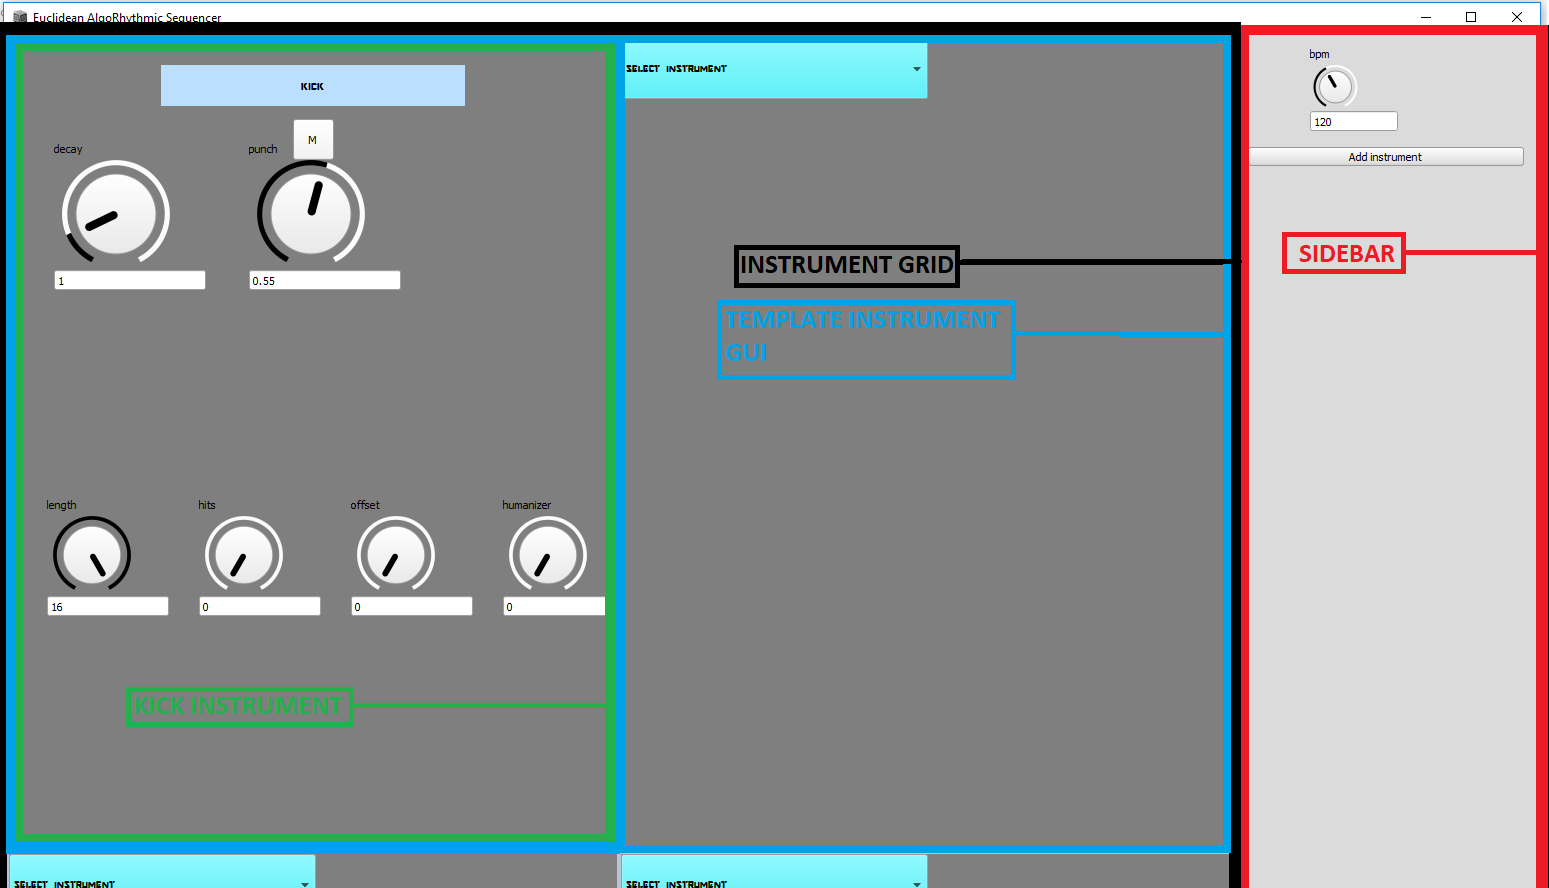
\includegraphics[height=10cm, width=15cm, keepaspectratio]{images/gui.png}
\caption{View of application}
\end{figure}\\
[2mm]
The graphical user interface has been developed following two guidelines: to be responsive and dynamic.\\
[2mm]
The responsiveness of a GUI means its adaptability to different screen sizes and formats. In order to achieve this goal, it has been decided to make a strong use of the composite pattern implemented in Supercollider.
The composite pattern is characterized by a given class A, that can contain a list of other instances of the same type A, thus creating a three-like structure. As an example, the root could be the application window, that contains other groups of elements, that can contain themselves other elements and so on…
Supercollider implements the composite pattern through the View class, in particular each GUI object must belong to a subclass of View.\\
[2mm]
View requires two arguments, the container of the element, and a set of parameters describing its bounds in term of pixels.\\
In the actual implementation each GUI component passes itself to the constructor of the children components, so that they can infer its dimensions and scale their size accordingly.\\
In the code snippet below, it is shown an example of this recurring pattern: a container, called instGrid, passes itself to its child component TemplateInstGUI. This behaviour is needed, because all the classes in the application that create GUI components, being subclasses of View, need the container View on which they must be attached to. It is also useful for the scaling purposes explained before.\\
[2mm]
\begin{lstlisting}[
  style      = SuperCollider-IDE,
  basicstyle = \scttfamily\small,
  caption    = {Generate View from main.scd},
  label = {lst:createGrid}
]
(
s.waitForBoot{(@\Suppressnumber@
//Code from main.scd
@\Reactivatenumber{159}@
instGrid = ScrollView.new(w,Rect(0,0, instGrid_width, w_height) );@\Suppressnumber@
//...
@\Reactivatenumber{173}@
slot1 = TemplateInstGUI.new.create(instGrid);
\end{lstlisting}

\begin{lstlisting}[
  style      = SuperCollider-IDE,
  basicstyle = \scttfamily\small,
  caption    = {Controller of TemplateInstGui},
  label = {lst:controlGrid}
]
TemplateInstGUI{
	var m, templateView;
	
	create{ arg instGrid;
		
		var instGrid_width = instGrid.bounds.width;
		var templateView_spacing = 7;//spacing between the various templateViews
		
		//CREATES THE CONTAINER "templateView"
		templateView = CompositeView.new(instGrid, Rect(0, 0, (instGrid_width/2) - templateView_spacing, (instGrid_width*2/3) - templateView_spacing ) );@\Suppressnumber@
		//...
		@\Reactivatenumber{30}@
	}
}
\end{lstlisting}

To ensure complete scalability of the GUI, in the main.scd script, the sizes of the screen are retrieved through a system call, and those quantities are used to scale every other portion of the GUI. Going up in the hierarchy of components and subcomponents we reach the main window that contains the whole application, which is proportional to the screen size. This implementation allows to have a user interface that scales with the screen dimensions.\\
[2mm]
In order to have a dynamic GUI, that allows the user to create, erase and replace instances of the various instruments, it was necessary to define a slot, which could host any different kind of instrument. Consequently, a way to abstract on the way each specific instrument is created, was needed.\\ 
The proposed solution makes use of the factory method patter, which is a common design pattern in object oriented programming. This enables writing of subclasses to change the way an object is created (to redefine which class to instantiate)\cite{DesignPattern:Gamma}. 
To implement it, it is necessary to make an abstraction on the way instrument objects that are created (Inst class) and provide a class that is responsible for the creation of such objects (Inst Factory).
The class diagram below depicts the simplified architecture for instruments creation and behaviour. The Supercollider classes are omitted for the sake of clarity.
\begin{figure}[htbp]
\centering
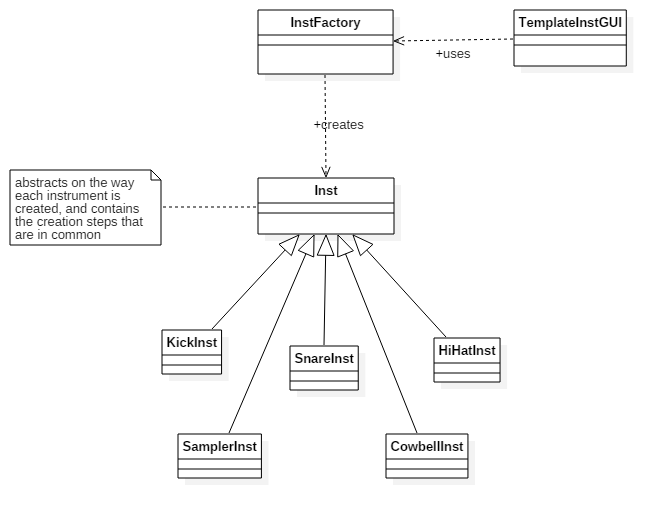
\includegraphics[height=5.4cm, width=12cm, keepaspectratio]{images/factory_pattern_uml.png}
\caption{Class diagram of the application}
\label{fig:uml}
\end{figure}

To show the advantages of such pattern, it will be shown how TemplateInstGUI is able to create and “host” a generic instrument, by using InstFactory, without worrying about the differences in the creation of each specific instrument. Since Supercollider does not have interfaces, like most object oriented programming languages, the abstraction is done by dividing the common creational step among the various instruments in the method  initializeSequencerGui  in the superclass Inst. This method is then called during the creation of instrument specific GUI elements in the createView method, in each instrument class. Here only the code for the kick instrument is shown, since the other instruments present a very similar code structure.

\begin{lstlisting}[
  style      = SuperCollider-IDE,
  basicstyle = \scttfamily\small,
  caption    = {TemplateInstGui Class},
  label = {lst:TemplateInstGui}
]
TemplateInstGUI{@\Suppressnumber@
	//...
	@\Reactivatenumber{5}@
	create{ | instGrid |@\Suppressnumber@
		//...
		@\Reactivatenumber{15}@
		m = PopUpMenu(templateView, Rect(0, 0, instGrid_width/4, instGrid_width/20));
		m.items = InstFactory.getInstuments;@\Suppressnumber@
		//...
		@\Reactivatenumber{22}@
		m.action = { arg menu;
			if(menu.item!="SELECT INSTRUMENT",
				{var inst = InstFactory.getIstance(menu.item);
					inst.createView(templateView);
			}, {});
		};
	}
}
\end{lstlisting}
\begin{lstlisting}[
  style      = SuperCollider-IDE,
  basicstyle = \scttfamily\small,
  caption    = {Factory of Instruments},
  label = {lst:InstFactoryClass},
  firstnumber = 33
]
InstFactory {

	classvar <>instrumentId=500;

	*getIstance{ | name |

		var instance = case

		{ name == "kick" }   { instance = KickInst.new}

		{ name == "kick808" } { instance = Kick808Inst.new }

		{ name == "snare" } { instance = SnareInst.new }

		{ name == "SOSsnare" } { instance = SOSsnareInst.new }

		{ name == "hi-hat" } { instance = HiHatInst.new }

		{ name == "sampler" }   { instance = SamplerInst.new }

		{ name == "cowbell" }   { instance = CowbellInst.new }

		{ name == "kalimba" }   { instance = KalimbaInst.new }

		{ name == "marimba" }   { instance = MarimbaInst.new }

		{ name == "SOShats"} { instance = SOShatsInst.new};

		instance.pdefId = this.prGenIstrumetId;
		^instance;

	}@\Suppressnumber@
	//...
	@\Reactivatenumber{67}@
}
\end{lstlisting}
\begin{lstlisting}[
  style      = SuperCollider-IDE,
  basicstyle = \scttfamily\small,
  caption    = {Instrument Abstract Class},
  label = {lst:InstAbstractClass},
  firstnumber = 69
]
Inst {@\Suppressnumber@
	//...
	@\Reactivatenumber{77}@
	/*initializeSequencerGui INITIATES THE GUI RELATIVE TO A GENERIC INSTRUMENT*/
	initializeSequencerGui { | instView |@\Suppressnumber@
		//SETTING COMMON GUI DIMENSIONS
		//SETTING INSTRUMENT LABEL
		//CREATING EUCLIDEAN RHYTHM CONTROLS
		//CREATING HUMANIZER CONTROLS
	@\Reactivatenumber{166}@
	}@\Suppressnumber@
	//...
	@\Reactivatenumber{194}@
}
\end{lstlisting}
\begin{lstlisting}[
  style      = SuperCollider-IDE,
  basicstyle = \scttfamily\small,
  caption    = {Kick Class},
  label = {lst:},
  firstnumber = 197
]
KickInst : Inst {@\Suppressnumber@
	//...
	@\Reactivatenumber{202}@
	/*CREATES THE INTRUMENT SPECIFIC GUI COMPONENTS, AFTER CREEATING THE COMPOSITE VIEW FOR THIS INSTRUMENT*/
	createView{ | templateView |

		instView = CompositeView.new(templateView, Rect(0, 0, templateView.bounds.width, templateView.bounds.height) );
		instView.background = Color.grey;

		super.initializeSequencerGui(instView);@\Suppressnumber@
		//...
		@\Reactivatenumber{240}@
	}@\Suppressnumber@
	//...
	@\Reactivatenumber{256}@
}
\end{lstlisting}
\end{document}